\documentclass[a4paper,10pt]{article}
\usepackage[utf8]{inputenc}
\usepackage[spanish]{babel}
\usepackage[affil-it]{authblk}
\usepackage{enumerate}
\usepackage{graphicx}
\usepackage{hyperref}
\usepackage{amsmath}
\usepackage{amssymb}
\usepackage{cancel}
\usepackage[usenames, dvipsnames]{color}
\usepackage{tikz}
\usepackage{multimedia}
\usepackage{subcaption} %Multiple images
\usepackage{multicol} % Multiple columns
\usepackage{float}
\usepackage{cleveref}
\usepackage[margin=1.4in]{geometry}
\usepackage[labelfont=bf]{caption}
\usetikzlibrary{calc}
\numberwithin{equation}{section}

%Columns separation
\setlength{\columnsep}{1cm}

%Indentation
\setlength{\parindent}{0ex}

%Multiple References

\usepackage{xparse}
\ExplSyntaxOn
\NewDocumentCommand{\mref}{m}{\quinn_mref:n {#1}}
\seq_new:N \l_quinn_mref_seq
\cs_new:Npn \quinn_mref:n #1
 {
  \seq_set_split:Nnn \l_quinn_mref_seq { , } { #1 }
  \seq_pop_right:NN \l_quinn_mref_seq \l_tmpa_tl
  ( % print the left parenthesis
  \seq_map_inline:Nn \l_quinn_mref_seq
    { \ref{##1},\nobreakspace } % print the first references
  \exp_args:NV \ref \l_tmpa_tl 
  ) 
 }
\ExplSyntaxOff


%Boxes

\newcommand*{\boxcolor}{blue}
\makeatletter
\renewcommand{\boxed}[1]{\textcolor{\boxcolor}{%
\tikz[baseline={([yshift=-1ex]current bounding box.center)}] \node [rectangle, minimum width=1ex,rounded corners,draw] {\normalcolor\m@th$\displaystyle#1$};}}
 \makeatother

%Constantes
\newcommand{\euler}{\mathrm{e}}
\newcommand{\im}{i}

%Lemas, teoremas, definiciones y pruebas
\newcommand{\definicion}{\textbf{Definición: }}
\newcommand{\lema}{\textbf{Lema: }}
\newcommand{\teorema}{\textbf{Teorema: }}
\newcommand{\prueba}{\textbf{Prueba: }}


%opening
\title{Mecánica Clásica Tarea \# 4}
\author{Favio Vázquez\thanks{Correo: favio.vazquezp@gmail.com}}\affil{Instituto de Ciencias Nucleares. Universidad Nacional Autónoma de México.}
\date{}

\begin{document}

\makeatletter
\def\@maketitle{%
  \newpage
  \null
  \vskip 2em%
  \begin{center}%
  \let \footnote \thanks
    {\Large\bfseries \@title \par}%
    \vskip 1.5em%
    {\normalsize
      \lineskip .5em%
      \begin{tabular}[t]{c}%
        \@author
      \end{tabular}\par}%
    \vskip 1em%
    {\normalsize \@date}%
  \end{center}%
  \par
  \vskip 1.5em}
\makeatother

\maketitle

\section{Problema 1}

Una partícula de masa $m_1$ se mueve a lo largo de una recta, otra de masa $m_2$ lo 
hace a lo largo de otra reta perpendicular a la primera. Las partículas interaccionan 
entre sí por medio de la gravedad. Encuentra las ecuaciones de movimiento. Usando 
una computadora trace una trayectoria en el espacio de configuración para algunas 
masas y condiciones iniciales.

\vspace{.3cm}

Suponga que $m_2=m_1+\epsilon$, donde $\epsilon$ es una cantidad pequeña. Encuentre 
las ecuaciones de movimiento a primer orden en $\epsilon$. Usando una computadora 
trace una órbita genérica para este caso.

\vspace{.3cm}

\underline{Solución:} \vspace{.3cm}

Para la primera parte del problema, desarrollaremos las ecuaciones de movimiento 
para un caso general, y trazaremos las trayectorias en el espacio de configuración
usando la computadora. Luego aplicaremos la condición de que $m_2=m_1+\epsilon$ y 
encontraremos las ecuaciones de movimiento a primer orden para $\epsilon$.

\vspace{.3cm}

En la figura de abajo se muestra la esquematización del problema que tratamos,

\begin{figure}[H]
\center
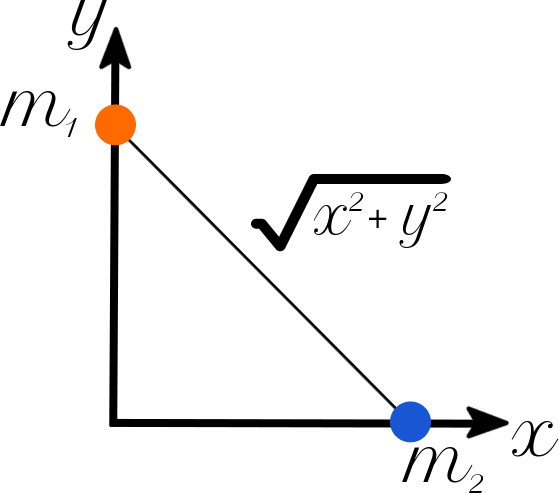
\includegraphics[scale=0.4]{problema1fig1}
\caption{Espacio de configuración del problema general para dos partículas $m_1$ y $m_2$,
ambas constreñidas a moverse en una recta, la una perpendicular a la otra.}
\label{fig:problema1fig1}
\end{figure}

Debido a que ambas partículas están constreñidas a moverse cada una en una recta, 
el espacio de configuración será el producto cartesiano de dos rectas, por lo tanto
tendrá dos dimensiones. Debido a la la configuración que planteamos es obvio que debemos
trabajar con coordenadas cartesianas para resolver el problema. Comencemos por un tratamiento
de las fuerzas que actúan sobre cada partícula; debido a que la única fuerza que 
actúa sobre ambas es la fuerza gravitacional, y debido a que ambas partículas se mueven
sobre una recta, únicamente debemos tomar la componente de la fuerza sobre la recta
para ambas partículas. Calculemos entonces la fuerza sobre cada partícula en coordenadas
cartesianas $(x,y)$, donde la distancia que las separa es $\sqrt{x^2+y^2}$, 
y obtendremos para la primera partícula

\begin{equation}
 F_x = - \frac{G m_1 m_2 x}{(x^2+y^2)^{3/2}},
\end{equation}

y para la segunda partícula

\begin{equation}
  F_y = - \frac{G m_1 m_2 y}{(x^2+y^2)^{3/2}},
\end{equation}

donde $G$ es la constante de gravitación universal. Es fácil ver que estas dos  fuerzas 
son derivables de un potencial, y ambas del mismo, que es el siguiente

\begin{equation}
 V(x,y) = - \frac{G m_1 m_2}{\sqrt{x^2+y^2}}.
\end{equation}

Por otra parte la energía cinética será

\begin{equation}
 T = \frac{1}{2} m_1 \dot{x}^2 + \frac{1}{2} m_2 \dot{y}^2 = \frac{1}{2} (m_1 \dot{x}^2 + m_2 \dot{y}^2)
\end{equation}

El sistema claramente es conservativo, ya que hemos encontrado un potencial que genere 
las fuerzas que actúan sobre las partículas. Podemos ahora escribir la función lagrangiana
$L = T - V$, 

\begin{equation}
 L = \frac{1}{2} (m_1 \dot{x}^2 + m_2 \dot{y}^2) +  \frac{G m_1 m_2}{\sqrt{x^2+y^2}}
\end{equation}

Y utilizando las ecuaciones de Lagrange, podemos encontrar las ecuaciones de movimiento. 

\vspace{.3cm}

Para $m_1$ tenemos,

\begin{equation}
 \frac{d}{dt} \frac{\partial L}{\partial \dot{x}} - \frac{\partial L}{\partial x} = 0,
\end{equation}

\begin{equation}
 m_1 \ddot{x} + \frac{G m_1 m_2 x}{(x^2+y^2)^{3/2}} = 0,
\end{equation}

Si dividimos por $m_1$ esta ecuación obtenemos que,

\begin{equation}
 \boxed{\ddot{x} + \frac{G m_2 x}{(x^2+y^2)^{3/2}} = 0.}
\end{equation}

Donde hemos llegado a la importante conclusión que el movimiento de la partícula $m_1$,
no depende de su masa, sino solamente la masa de la segunda partícula.

\vspace{.3cm}

Para $m_2$ tenemos,

\begin{equation}
 \frac{d}{dt} \frac{\partial L}{\partial \dot{y}} - \frac{\partial L}{\partial y} = 0,
\end{equation}

\begin{equation}
 m_2\ddot{y} + \frac{G m_1 m_2 y}{(x^2+y^2)^{3/2}} = 0.
\end{equation}

Si dividimos por $m_2$ esta ecuación obtenemos que,

\begin{equation}
 \boxed{\ddot{y} + \frac{G m_1 y}{(x^2+y^2)^{3/2}} = 0.}
\end{equation}

Donde llegamos a la misma conclusión que para la primera partícula. 
Hemos encontrado las ecuaciones de movimiento para $m_1$ y $m_2$. 
Para poder resolver numéricamente conviene escribir estas ecuaciones como,

\begin{align}
 \xi &= \dot{x}, \\ 
 \dot{\xi} &= \frac{G m_2 x }{(x^2+y^2)^{3/2}}.
\end{align}

Y,

\begin{align}
 \chi &= \dot{y}, \\
 \dot{\chi} &= - \frac{G m_1 y }{(x^2+y^2)^{3/2}}.
\end{align}

Para trazar las trayectorias hemos utilizado en todas las
gráficas que inicialmente $\dot{\xi} = \dot{\chi} = 0$, y hemos probado varias 
combinaciones para las posiciones iniciales y las masas de las partículas. Los códigos 
con los que realicé los gráficos son libres y se encuentran en un NoteBook de Python,
en el siguiente \href{https://github.com/FavioVazquez/MecanicaClasica-PCF/blob/master/Tarea4/Problema\%201.ipynb}{\color{blue}{.::link::.}}

\begin{multicols}{2}
\begin{figure}[H]
\begin{subfigure}{.4\textwidth}
\centering
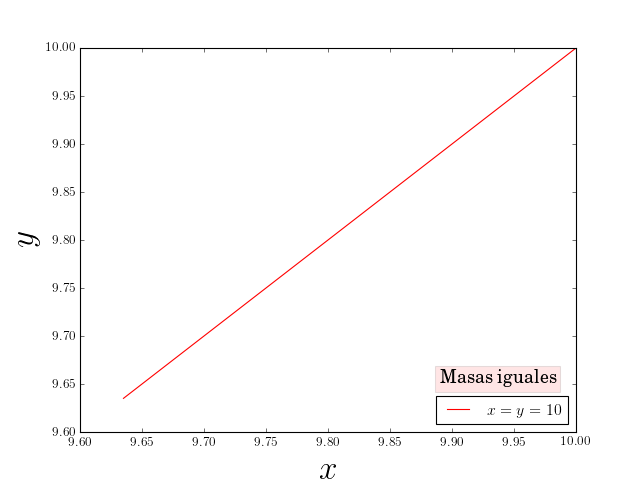
\includegraphics[scale=0.3]{problema1fig2}
\label{fig:problema1fig2}
\end{subfigure}

\begin{subfigure}{.4\textwidth}
\centering
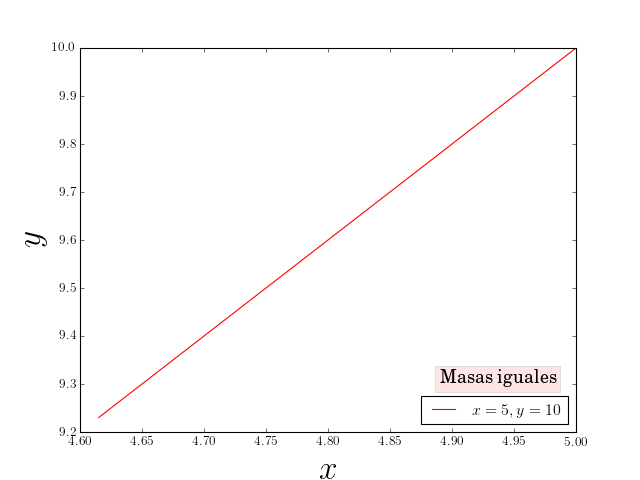
\includegraphics[scale=0.3]{problema1fig3}
\label{fig:problema1fig3}
\end{subfigure}
\end{figure}

\begin{figure}[H]
\begin{subfigure}{.4\textwidth}
\centering
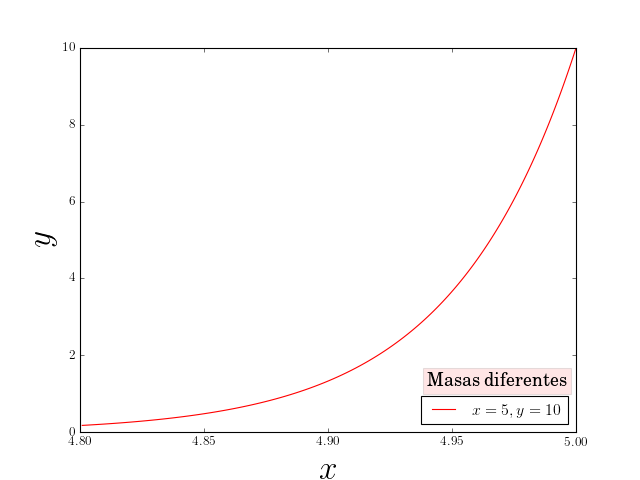
\includegraphics[scale=0.3]{problema1fig4}
\label{fig:problema1fig4}
\end{subfigure}

\begin{subfigure}{.4\textwidth}
\centering
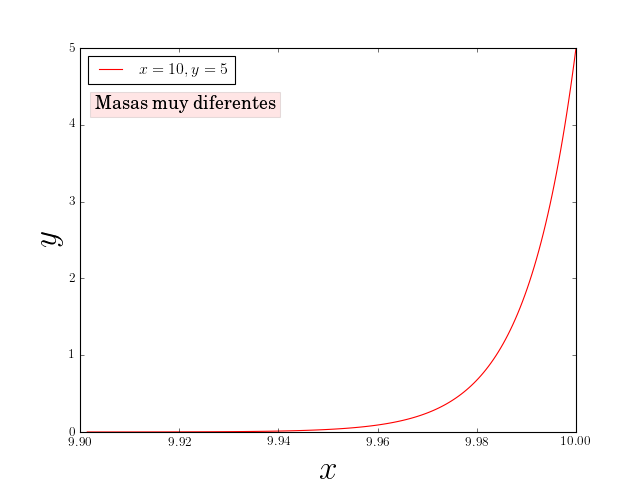
\includegraphics[scale=0.3]{problema1fig5}
\label{fig:problema1fig5}
\end{subfigure}
\end{figure}
\end{multicols}

Ahora utilizando el hecho de que $m_2 = m_1 + \epsilon$, primero la energía cinética será

\begin{equation}
 V(x,y) = - \frac{G m_1 (m_1 + \epsilon)}{\sqrt{x^2+y^2}}. 
\end{equation}

Y la energía cinética,

\begin{equation}
  T = \frac{1}{2} [m_1 \dot{x}^2 +  (m_1+\epsilon) \dot{y}^2].
\end{equation}

Y la lagrangiana será,

\begin{equation}
 L = \frac{1}{2} [m_1 \dot{x}^2 +  (m_1 + \epsilon) \dot{y}^2] + 
 \frac{G m_1 (m_1 + \epsilon)}{\sqrt{x^2+y^2}}.
\end{equation}

Las ecuaciones de movimiento serán,

\begin{equation}
 m_1 \ddot{x} + \frac{G m_1 (m_1 + \epsilon) x}{(x^2+y^2)^{3/2}} = 0,
\end{equation}

\begin{equation}
 (m_1 + \epsilon) \ddot{y} + \frac{G m_1 (m_1 + \epsilon) y}{(x^2+y^2)^{3/2}} = 0.
\end{equation}


o,

\begin{equation}
\boxed{\ddot{x} + \frac{G (m_1 + \epsilon) x}{(x^2+y^2)^{3/2}} = 0,}
\end{equation}

\begin{equation}
 \boxed{\ddot{y} + \frac{G m_1 y}{(x^2+y^2)^{3/2}} = 0.}
\end{equation}

Que son las ecuaciones de movimiento para primer orden en $\epsilon$.

\vspace{.3cm}

Para trazar las trayectorias en este caso hemos utilizado distintas condiciones iniciales
para la posición de las partículas.

\begin{multicols}{2}
\begin{figure}[H]
\centering
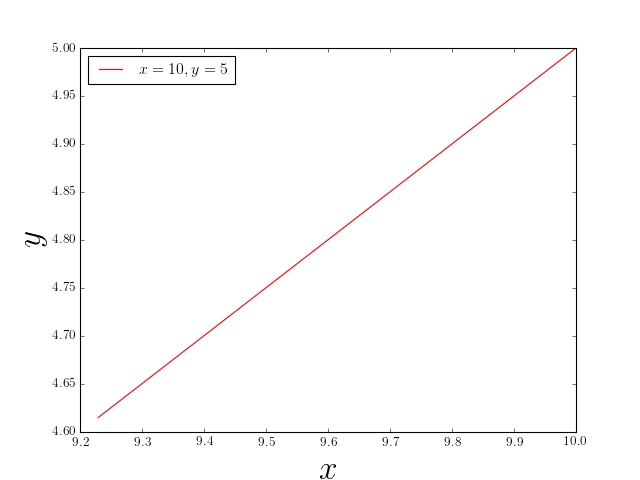
\includegraphics[scale=0.33]{problema1fig6}
\label{fig:problema1fig6}
\end{figure}

\begin{figure}[H]
\centering
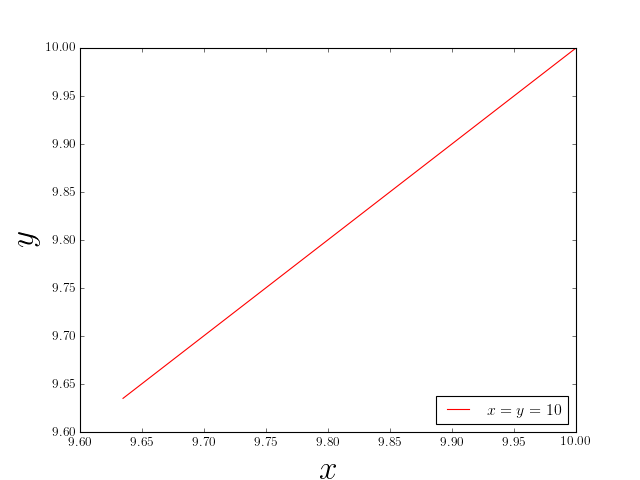
\includegraphics[scale=0.33]{problema1fig7}
\label{fig:problema1fig7}
\end{figure}
\end{multicols}

\newpage

\section{Problema 2}

Encuentre las ecuaciones de movimiento del péndulo doble usando únicamente métodos 
vectoriales. El péndulo doble tiene las dos masas iguales y las dos longitudes iguales.
Usando una computadora trace la trayectoria $(\theta_1$ vs $\theta_2)$ cuando las 
condiciones iniciales son

\begin{align*}
 \theta_1 &= \frac{\pi}{2} \\
 \theta_2 &= \pi \\
 \dot{\theta_1} &= 0 \\
 \dot{\theta_2} &= 0 
\end{align*}

\vspace{.3cm}

\underline{Solución:} \vspace{.3cm}

En la figura de abajo se muestra un diagrama del problema, 

\begin{figure}[H]
\center
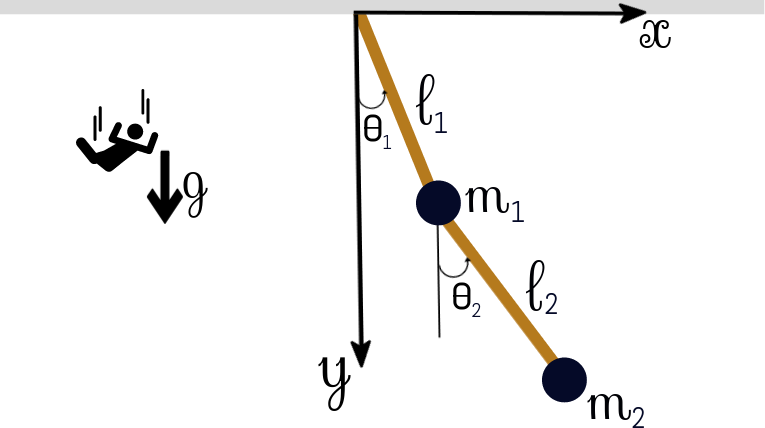
\includegraphics[scale=0.4]{problema2fig1}
\caption{Péndulo doble. Como muestra el muñequito la gravedad va dirigida hacia 
abajo.}
\label{fig:problema2fig1}
\end{figure}


Consideraremos un caso general en el cual las longitudes y masas pueden ser diferentes,
y luego haremos la simplificación que el enunciado indica. El doble péndulo consiste 
en dos masa $m_1$ y $m_2$ conectadas por barras sin masa de longitudes $l_1$ y $l_2$,
sujetas a la fuerza de gravedad, y constreñidas por las junturas entre las varas
a moverse en un plano. Escogeremos un sistema de coordenadas con el origen en el 
tope del punto de suspensión, y el eje $x$ como un eje horizontal en el plano del 
movimiento, y el eje $y$ hacia abajo, de manera tal que las fuerzas de gravedad 
tengan componentes positivas.

\vspace{.3cm}

El sistema tiene dos partículas, digamos que con posiciones $\mathbf{r_1}$ y $\mathbf{r_2}$,
cada una con componentes $(x_i,y_i,z_i)$. Como hemos dicho el sistema se moverá 
en el plano de $x-y$, por lo tanto consideraremos esto como una restricción, ligadura,
o constricción; entonces habrá una de estas constricciones para cada partícula, y 
hay otras dos más, el hecho de que cada barra tiene una longitud constante. Podemos 
escribir estas constricciones como:

\begin{align}
 z_1 &= 0, \\
 z_2 &= 0, \\
 |\mathbf{r_1}| &= l_1, \\
 |\mathbf{r_2} - \mathbf{r_1}| &= l_2.
 \label{eq:pendu1}
\end{align}

Entonces para el caso que consideremos del péndulo doble, tendremos solamente, dos (2)
grados de libertad, debido a que los originales seis (6) se reducen por las cuatro (4)
constricciones al movimiento que consideramos. 

\vspace{.3cm}

El lector familiarizado con este problema, ya clásico de la mecánica, recordará que en 
la formulación lagrangiana de este problema, las coordenadas generalizadas más utilizadas
y que simplifican la solución del problema son $\theta_1$ y $\theta_2$, por lo tanto
las ecuaciones de movimiento se expresarán en término de las mismas, para así poder tener 
una comparación directa con el análisis vectorial del problema que haremos, con el escalar
que se trabaja en la formulación lagrangiana. Podemos encontrar expresiones para $\mathbf{r_1}$ y $\mathbf{r_2}$ en términos 
de los dos ángulos $\theta_1$ y $\theta_2$ (hemos suprimido los vectores unitarios 
ya que no influirán en el desarrollo del problema, pero debe aclararse que están allí
para consistencia vectorial):

\begin{align}
 \mathbf{r_1} &= l_1\sen{\theta_1} + l_1\cos{\theta_1} \\
 \mathbf{r_2} &= \mathbf{r_1} +  l_2\sen{\theta_2} + l_2\cos{\theta_2}
 \label{eq:pendu2}
\end{align}

Ahora podemos encontrar los vectores de velocidad y aceleración en término de $\theta_1$ y $\theta_2$,
para $m_1$,

\begin{equation}
 \dot{\mathbf{r_1}} = \mathbf{v_1} = l_1 \dot{\theta_1} \cos{\theta_1} - l_1 \dot{\theta_1} \sen{\theta_1} = l_1 \dot{\theta_1}(\cos{\theta_1} - \sen{\theta_1}),
 \label{eq:pendu3}
\end{equation}

\begin{align}
\begin{split}
 \ddot{\mathbf{r_1}} = \mathbf{a_1} &= l_1 \ddot{\theta_1} \cos{\theta_1} - l_1 \dot{\theta_1}^2 \sen{\theta_1} - l_1 \ddot{\theta_1} \sen{\theta_1} - l_1 \dot{\theta_1}^2 \cos{\theta_1}, \\
 &=  l_1 \ddot{\theta_1} (\cos{\theta_1} - \sen{\theta_1}) - l_1 \dot{\theta_1}^2 (\cos{\theta_1} +  \sen{\theta_1}),
 \label{eq:pendu4}
\end{split}
\end{align}

y para $m_2$

\begin{equation}
 \dot{\mathbf{r_2}} = \mathbf{v_2} = \mathbf{v_1} + l_2 \dot{\theta_2} \cos{\theta_2} - l_2 \dot{\theta_2} \sen{\theta_2} = l_2 \dot{\theta_2}(\cos{\theta_2} - \sen{\theta_2}),
 \label{eq:pendu5}
\end{equation}

\begin{align}
\begin{split}
 \ddot{\mathbf{r_1}} = \mathbf{a_2} &= \mathbf{a_1} + l_2 \ddot{\theta_2} \cos{\theta_2} - l_2 \dot{\theta_2}^2 \sen{\theta_2} - l_1 \ddot{\theta_2} \sen{\theta_2} - l_2 \dot{\theta_2}^2 \cos{\theta_2}, \\
 &= \mathbf{a_1} + l_2 \ddot{\theta_2} (\cos{\theta_2} - \sen{\theta_2}) - l_2 \dot{\theta_1}^2 (\cos{\theta_2} +  \sen{\theta_2}),
 \label{eq:pendu6}
\end{split}
\end{align}

Para poder construir las ecuaciones de movimiento en la metodología vectorial necesitamos 
conocer el sentido, dirección y magnitud de las fuerzas que actúan sobre las partículas 
en consideración. En este caso las fuerzas que actúan para $m_1$ son la tensión de las 
dos cuerdas (que llamaremos $\mathbf{T_1}$ y $\mathbf{T_2}$ respectivamente), y la gravedad.
La tensión de la cuerda $l_1$, sobre $m_1$ actúa lo largo de $-\mathbf{r_1}$, y la tensión 
de la cuerda $l_2$ actúa a lo largo de ($\mathbf{r_2} - \mathbf{r_1}$), entonces podemos 
escribir la fuerza $\mathbf{F_1}$ como

\begin{equation}
 \mathbf{F_1} = T_1 \frac{-\mathbf{r_1}}{|\mathbf{r_1}|} + T_2 \frac{\mathbf{r_2} - \mathbf{r_1}}{|\mathbf{r_2} -\mathbf{r_1}|}
	      + m_1 \mathbf{g} = - \frac{T_1}{l_1} \mathbf{r_1} + \frac{T_1}{l_1} (\mathbf{r_2} - \mathbf{r_1}) + m_1 \mathbf{g}.
\end{equation}

Las fuerzas sobre $m_2$ son la tensión de la cuerda $l_2$ a lo largo de -($\mathbf{r_2} - \mathbf{r_1}$)
y la gravedad,

\begin{equation}
 \mathbf{F_2} = T_2 \frac{-(\mathbf{r_2} - \mathbf{r_1})}{|\mathbf{r_2} -\mathbf{r_1}|}
	      + m_2 \mathbf{g} = - \frac{T_2}{l_2} (\mathbf{r_2} -\mathbf{r_1}) + m_2 \mathbf{g}.
\end{equation}

Estamos ahora en posición para escribir las ecuaciones de movimiento para el péndulo 
doble utilizando la segunda ley de Newton en cada partícula, $\mathbf{F_i} = m_i \ddot{\mathbf{r_i}}$:

\begin{align}
 m_1 \ddot{\mathbf{r_1}} &= - \frac{T_1}{l_1} \mathbf{r_1} + \frac{T_1}{l_1} (\mathbf{r_2} - \mathbf{r_1}) + m_1 \mathbf{g}, \\
 m_2 \ddot{\mathbf{r_2}} &= - \frac{T_2}{l_2} (\mathbf{r_2} -\mathbf{r_1}) + m_2 \mathbf{g}.
\end{align}

Estas ecuaciones no son muy esclarecedoras del problema al cual nos enfrentamos, y ahora 
es claro por qué debemos expresar las mismas para $\theta_1$ y $\theta_2$, debido que como 
veremos estas se convertirán en cuatro ecuaciones diferenciales para cuatro incógnitas, 
$\theta_1$, $\theta_2$, $T_1$ y $T_2$. Escribimos entonces las ecuaciones de movimiento 
para las dos partículas en sus componentes en el plano\footnote{Acá utilizaremos la muy conocida separación
de componentes de fuerzas de la mecánica newtoniana} ($x-y$), utilizando (\ref{eq:pendu3}) y (\ref{eq:pendu4}) y 
la figura (\ref{fig:problema2fig1}),

Para $m_1$,

\begin{align}
 m_1 l_1 (\ddot{\theta_1}\cos{\theta_1} - \dot{\theta_1}^2\sen{\theta_1}) &= - T_1 \sen{\theta_1} + T_2 \sen{\theta_2}, \\
 -m_1 l_1 (\ddot{\theta_1}\sen{\theta_1} + \dot{\theta_1}^2\cos{\theta_1}) &= - T_1 \cos{\theta_1} + T_2 \cos{\theta_2} + m_1 g.
\end{align}

Para $m_2$,

\begin{align}
 m_2(l_1\ddot{\theta_1}\cos{\theta_1} - l_1\dot{\theta_1}^2\sen{\theta_1} + l_2\ddot{\theta_2}\cos{\theta_2} - l_2\dot{\theta_2}^2\sen{\theta_2})
 &= - T_2 \sen{\theta_2}, \\
 - m_2(l_1\ddot{\theta_1}\sen{\theta_1} + l_1\dot{\theta_1}^2\cos{\theta_1} + l_2\ddot{\theta_2}\sen{\theta_2} - l_2\dot{\theta_2}^2\cos{\theta_2})
 &= - T_2 \cos{\theta_2} + m_2 g.
\end{align}

Haciendo uso de algunas identidades trigonométricas como $\cos^2{\theta} +  \sen^2{\theta} = 1$, y
$\sen{\theta_2}\cos{\theta_1} - \cos{\theta_2}\sen{\theta_1} = \sen{(\theta_2 - \theta_1)}$, 
y un largo trabajo algebraico que no aportaría nada colocarlo explícitamente en esta tarea,
llegamos a que las ecuaciones de movimiento pueden escribirse como:

\begin{align}
  \label{eq:pendu7} % la de abajo
 l_1\ddot{\theta_1} &= \frac{T_2}{m_1}\sen{\theta_2 - \theta_1} - g \sen{\theta_1}, \\
 \label{eq:pendu8} % la de abajo
 l_1\dot{\theta_1}^2 &= \frac{T_1}{m_1} - \frac{T_2}{m_1}\cos{(\theta_2 - \theta_1)} - g \cos{\theta_1}, \\
  \label{eq:pendu9} % la de abajo
 l_2\ddot{\theta_2} &= - \frac{T_2}{m_1}\sen{\theta_2 - \theta_1}, \\
  \label{eq:pendu10} % la de abajo
 l_2\dot{\theta_2}^2 &= \frac{T_2}{m_2} - \frac{T_2}{m_1} - \frac{T_1}{m_1}\cos{(\theta_2 - \theta_1)}.
 \end{align}

Debido a que las ecuaciones no contienen derivadas de $T_1$ y $T_2$, la mejor manera 
de escribir las ecuaciones para el análisis numérico que realizaremos, es obtener 
dos ecuaciones diferenciales para $\theta_1$ y $\theta_2$ sin los términos de $T_1$
y $T_2$. Para hacer eso hacemos uso de (\ref{eq:pendu7}) y (\ref{eq:pendu9}), y 
obtenemos que 

\begin{equation}
 T_1 = - m_1 \frac{l_2\ddot{\theta_2}}{\sen{(\theta_2 - \theta_1)}},
\end{equation}

\begin{equation}
 T_2 = m_1 \frac{l_1 \ddot{\theta_1} + g \sen{\theta_1}}{\sen{(\theta_2 - \theta_1)}}.
\end{equation}

Sustituimos estas expresiones, primero en \mref{eq:pendu8} y obtenemos 

\begin{align*}
 l_1 \dot{\theta_1}^2 &= \frac{T_1}{m_1} - \frac{T_2}{m_1}\cos{(\theta_2 - \theta_1)} - g \cos{\theta_1}, \\
		      &= - \frac{l_2\ddot{\theta_2}}{\sen{(\theta_2 - \theta_1})}
		         -   \frac{l_1 \ddot{\theta_1} + g \sen{\theta_1}}{\sen{(\theta_2 - \theta_1)}}\cos{(\theta_2 - \theta_1)}
		         - g \cos{\theta_1},
\end{align*}

\begin{equation}
 \boxed{\therefore l_2 \ddot{\theta_2} + l_1 \ddot{\theta_1}\cos{(\theta_2 - \theta_1)} 
 + l_1 \dot{\theta_1}^2\sen{(\theta_2 - \theta_1)} + g \sen{\theta_2} = 0.}
\end{equation}

ahora en \mref{eq:pendu10} y obtenemos,

\begin{equation}
 \boxed{(m_1 + m_2) l_1 \ddot{\theta_1} + m_2 l_2 \ddot{\theta_2}\cos{(\theta_2 - \theta_1)}
 - m_2 l_2 \dot{\theta_2}^2 \sen{(\theta_2 - \theta_1)} + (m_1 + m_2)g\sen{\theta_1} = 0.}
\end{equation}

\vspace{.3cm}

Que son las conocidas ecuaciones de movimiento para un péndulo doble. Para que sea más
fácil el análisis computacional, llamemos a $\omega_1 = \dot{\theta_1}$, y 
$\omega_2 = \dot{\theta_2}$, las velocidades respectivas velocidades angulares,
con lo cual

\begin{equation}
 \omega_1 = \dot{\theta_1}
 \label{eq:pendu11}
\end{equation}

\begin{equation}
 \omega_2 = \dot{\theta_2}
 \label{eq:pendu12}
\end{equation}

\begin{equation}
 l_2 \dot{\omega_2} + l_1 \dot{\omega_1} \cos{(\theta_2 - \theta_1)} + l_1 \omega_1^2
 \sen{(\theta_2 - \theta_1)} + g \sen{\theta_2} = 0
 \label{eq:pendu13}
\end{equation}

\begin{equation}
 (m_1 + m_2)l_1 \dot{\omega_1} + m_2 l_2 \dot{\omega_2} \cos{(\theta_2 - \theta_1)}
 - m_2 l_2 \omega_2^2 \sen{(\theta_2 - \theta_1)} + (m_1 + m_2)g\sen{\theta_1} = 0 
 \label{eq:pendu14}
\end{equation}

El paso siguiente es puramente manipulación algebraica, la cual cubriría más de una 
página de puras ecuaciones que no suman a la demostración que queremos hacer, simplemente
lo que se hace es despejar $\dot{\omega_2}$ de \mref{eq:pendu13}, y luego se sustituye 
en \mref{eq:pendu14}, y luego se despeja $\dot{\omega_1}$ de \mref{eq:pendu14}, y luego se sustituye 
en \mref{eq:pendu13}, y obtendremos lo siguiente (hemos definido $\Delta = \theta_2 - \theta_1$):

\begin{align}
\begin{split}
\dot{\omega_1} &= \\
   &\frac{m_2 l_1 \omega_1^2 \sen{\Delta}\cos{\Delta}
 + m_2 g \sen{\theta_2}\cos{\Delta}-m_2 l_2 \omega_2^2\sen{\Delta} 
 +(m_1 + m_2)g \sen{\theta_1}}{(m_1 + m_2) l_1 - m_2 l_1 \cos^2{\Delta}},
\end{split}
 \end{align}

y

\begin{align}
\begin{split}
\dot{\omega_2} &= \\
   &\frac{m_2 l_2 \omega_2^2 \sen{\Delta}\cos{\Delta}
 + (m_1 + m_2)(g \sen{\theta_1}\cos{\Delta} - l_1 \omega_1^2\sen{\Delta}
 - g\sen{\theta_2})}{(m_1 + m_2) l_1 - m_2 l_2 \cos^2{\Delta}},
\end{split}
 \end{align}

Resolveremos estas ecuaciones diferenciales numéricamente utilizando varias librerías 
de Python, la primera es NumPy\footnote{\href{http://www.numpy.org/}{http://www.numpy.org/}},
que nos permite utilizar funciones trigonométricas y definir espacios algebraicos para 
las soluciones, la segunda es SciPy\footnote{\href{http://www.scipy.org/}{http://www.scipy.org/}},
para encontrar las soluciones numéricas a las ecuaciones y MatplotLib\footnote{
\href{http://matplotlib.org/}{http://matplotlib.org/}} para hacer los gráficos que 
veremos a continuación. Todo el código que realicé para la solución de este problema,
se encuentra en un repositorio público de GitHub y está disponible para su uso, reproducción
y consulta; el mismo se encuentra en un NoteBook de Python para su simple visualización,
pero en caso de querer el código en Python, envíenme un correo o solicítenlo por el 
repositorio. El repositorio completo se encuentra en \href{https://github.com/FavioVazquez/MecanicaClasica-PCF}{\color{blue} este link},
y particularmente el NoteBook de este problema en \href{https://github.com/FavioVazquez/MecanicaClasica-PCF/blob/master/Tarea4/Problema\%202.ipynb}{\color{blue} este link}.

\vspace{.3cm}

El diagrama completo del sistema, para las condiciones iniciales
del enunciado, se anexará en el correo, y también se encuentra en el 
repositorio. Cabe destacar que el código para realizar esta simulación en su mayoría 
fue recopilado de un ejemplo de MatplotLib, con algunas mejoras que realizamos aparte 
de que puede correr en un NoteBook de forma dinámica debido a algunos parámetros
que agregamos al código.

\vspace{.3cm}

Dibujaremos ahora varias combinaciones para el sistema, las cuales nos pintan 
una imagen completa del movimiento del mismo.

\begin{figure}[H]
\center
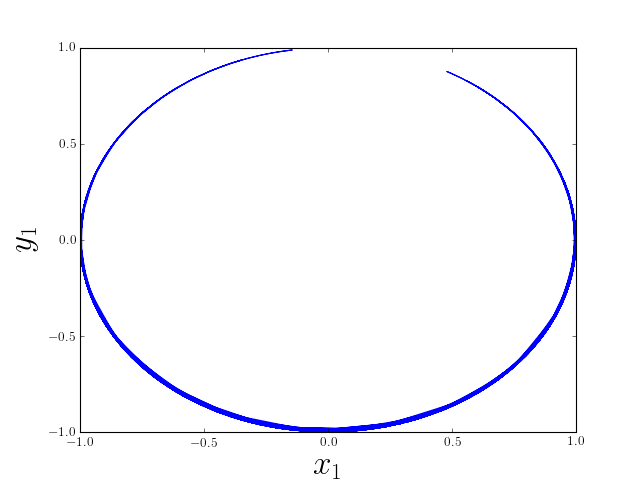
\includegraphics[scale=0.5]{problema2fig2}
\caption{$y_1$ vs $x_1$}
\label{fig:problema2fig2}
\end{figure}

\begin{figure}[H]
\center
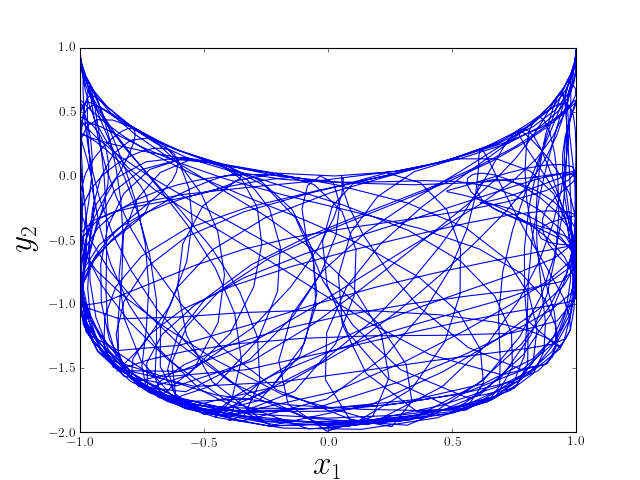
\includegraphics[scale=0.5]{problema2fig3}
\caption{$y_2$ vs $x_1$}
\label{fig:problema2fig3}
\end{figure}

\begin{figure}[H]
\center
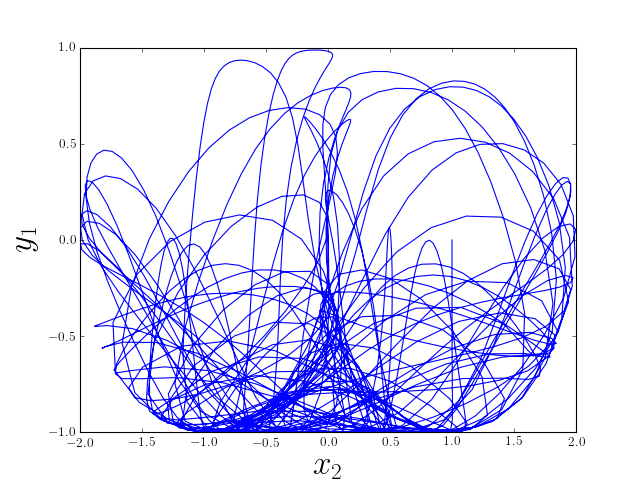
\includegraphics[scale=0.5]{problema2fig4}
\caption{$y_1$ vs $x_2$}
\label{fig:problema2fig4}
\end{figure}

\begin{figure}[H]
\center
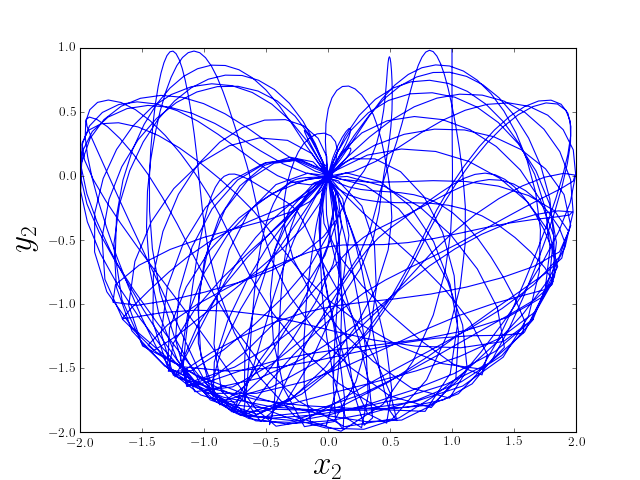
\includegraphics[scale=0.5]{problema2fig5}
\caption{$y_2$ vs $x_2$}
\label{fig:problema2fig5}
\end{figure}

\begin{figure}[H]
\center
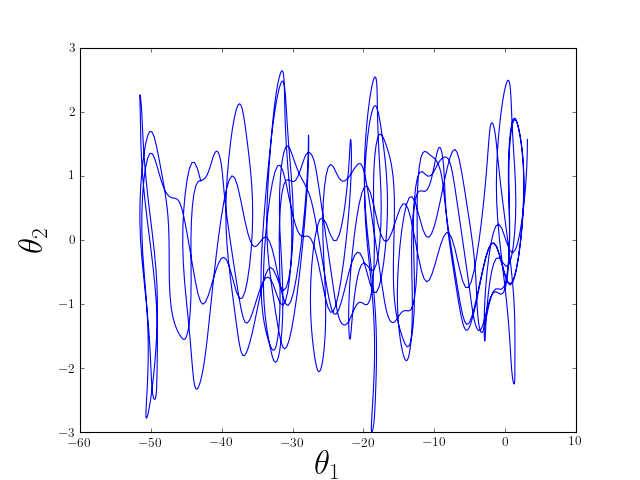
\includegraphics[scale=0.5]{problema2fig6}
\caption{$\theta_2$ vs $\theta_1$}
\label{fig:problema2fig6}
\end{figure}

Vemos entonces una gran concordancia con la simulación completa del péndulo doble y las 
gráficas de distintas proyecciones del movimiento, claramente se ve que en la masa 
$m_1$ se mueve en un círculo y la masa $m_2$ describe el movimiento caótico
tan conocido de este sistema.

\section{Problema 3}

Se encuentran un compañero de la prepa que no veían desde que salieron de ella. El 
amigo estudio derecho y le ha ido muy bien; se toman un café y cuando le dicen que 
estudiaron física el se pone contento y les dice: ``que bien, mira siempre he tenido
la curiosidad de saber qué son esas cosas que ustedes tanto usan y admira: los 
tensores, dime ¿qué son?''. Escriba en media cuartilla la respuesta que le darían 
a su compañero de la prepa que estudió derecho.

\vspace{.3cm}

\underline{Solución:} \vspace{.3cm}

Supongamos que mi amigo se llama Roger\footnote{Lo hago en alusión a mi matemático (vivo)
preferido, Roger Penrose.}. Comencemos la charla:

\vspace{.3cm}

\textbf{\color{ForestGreen}Roger}: Epa Favio, entonces los tensores, dime ¿qué son?

\textbf{\color{Blue}Favio}: Bueno Roger, los tensores son unas entidades matemáticas, pero
será más fácil describirte qué son en términos físico-matemáticos para usar un poco la 
intuición que a veces puede ser de mucha ayuda. En la física nos gusta ser precisos con 
la forma en que expresamos, representamos y medimos cantidades, y los tensores nos ayudan
mucho en esto. Supongamos que te pregunto, cuántos pesos llevas contigo, ¿qué me responderías?

\textbf{\color{ForestGreen}Roger}: Eh..., déjame revisar..., ¡ajá!, 300.

\textbf{\color{Blue}Favio}: Perfecto, lo que dices responde satisfactoriamente lo que te 
pregunté, el solo número 300 bastó para proveer la información que buscaba. Ahora, si yo
te preguntara cuán lejos queda tu casa de donde estamos, y me respondes ``20'', te miraría
un poco desconcertado y te preguntaría ``¿20 qué?'', claramente para responder a esta 
pregunta necesitarías darme más información, por ejemplo, ``20 km'', ahora que le has 
dado nombre a 20, representa una cantidad de kilómetros. Pero con esta información, 
¿crees que llegaría a tu casa desde acá?.

\textbf{\color{ForestGreen}Roger}: Eh..., no creo. ¿Tendría que decirte que dirección tomar no?

\textbf{\color{Blue}Favio}: Exacto Roger. Si me dijeras camina 20 km hacia el norte, entonces 
ya que me has dado una información direccional adicional con la que probablemente llegue a tu casa,
o al menos iría en el sentido correcto. En física, matemáticas e ingeniería le decimos 
a estas cantidades con nombre y dirección ``vectores''. Ah, y por cierto, a las primeras 
cantidades con nombre y sin dirección les llamamos ``escalares''. Ya con estas nociones 
puedo decirte un poquito sobre los tensores, aunque la intuición no será tan fácil
ahora de utilizar.

\textbf{\color{ForestGreen}Roger}: Ok, ¡pero apúrate por favor que ya tengo que ir a clase de 
derecho civil!

\textbf{\color{Blue}Favio}: Jajaja, bueno Roger, me apuraré. Con los vectores y escalares
podemos hacer una serie de operaciones bien definidas, como sumarlos, multiplicarlos, restarlos,
dividirlos, y otras. Aunque no es muy riguroso como te lo diré, aquí va. Si multiplicas 
un vector por un escalar obtienes otro vector con una magnitud distinta pero con 
la misma dirección; si multiplicas un vector por otro vector puedes obtener o un escalar,
lo que llamamos el producto punto o escalar, o un vector con el llamado producto cruz o 
vectorial, pero este nos limita a cambiar su dirección en ángulos de $90^\circ$. ¿Que tal 
si queremos cambiar la magnitud y la dirección de un vector arbitrariamente?, para ello
necesitamos una nueva entidad matemática, y estos son los tensores. Entonces un tensor 
es una entidad matemática muy útil cuando queremos expresar cantidades que tienen una 
magnitud pero pueden tener varias direcciones. ¿Me sigues?

\textbf{\color{ForestGreen}Roger}: ¡Sí claro continúa!

\textbf{\color{Blue}Favio}: ¡Ajá!, bueno estos son necesarios en las teorías 
más elegantes e interesantes de la física y matemática, y nos permiten escribir de forma
muy compacta artículos que tomarían toda una resma de papel, porque hay algo muy bonito,
los escalares de los que te hablé son tensores de orden 0, y los vectores son 
tensores de orden 1, ¡ahora solo con un concepto podemos capturar varios! Aparte que representan cantidades
complicadas como la gravedad, el estrés de los materiales, permeabilidad en materiales 
complejos y muchas otras cosas que te podría mencionar en otro momento. Bueno Roger, espero
que esta pequeña introducción hayas entendido un poco mejor qué son los tensores.

\textbf{\color{ForestGreen}Roger}: ¡Gracias Favio!, me quedó un poco más claro y ahora tengo una
idea de qué son. Luego leeré un poco más para complementar lo que me dices. Espero 
verte pronto para hacerte otras preguntas, una de ellas es, ¿qué es un Twistor? Jaja,
chao...

\textbf{\color{Blue}Favio}: ¡Jajaja chao!, para esa pregunta si necesitaré que me brindes 
el almuerzo, y vengas con tiempo porque no será tan fácil. ¡Éxitos!

\section{Problema 4}

Demuestre que si la torca aplicada sobre un cuerpo rígido simétrico está a lo largo 
del eje de simetría (digamos que el eje $z$), entonces $\omega_x^2 + \omega_y^2$ es 
una constante.

\vspace{.3cm}

\underline{Solución:} \vspace{.3cm}

Comencemos escribiendo la expresión general para las ecuaciones de Euler para un 
cuerpo rígido\footnote{Ver siguiente problema para una descripción más completa 
de las ecuaciones de Euler.}, en el cual pueden existir torques actuando sobre el,

\begin{equation}
 (I_i - I_j) \omega_i \omega_j \sum_k (I_k\dot{\omega_k}- \tau_k) \varepsilon_{ijk} = 0.
\end{equation}

Donde $I_j$ es el tensor de inercia para la coordenada $j$, $\omega_j$ es la velocidad
angular para la coordenada $j$, $\tau_j$ es el torque aplicado sobre la coordenada 
$j$ y $\varepsilon_{ijk}$ es el símbolo de permutación, también conocido como la 
densidad de \emph{Levi-Civita}, que para el lector no familiarizado está definido 
por 

\begin{align*}
 \varepsilon_{ijk} = \left\{\def\arraystretch{1.2}%
  \begin{array}{@{}c@{\quad}l@{}}
     &0 \quad \text{\hspace{.1cm} si cualquier índice es igual a otro índice}, \\
    &+1 \quad \text{si $i,j,k$ forman una permutación par de 1,2,3}, \\
    &-1 \quad \text{si $i,j,k$ forman una permutación impar de 1,2,3}.
  \end{array}\right.
\end{align*}

Entonces las ecuaciones de Euler toman la siguiente forma para un cuerpo rígido
de tres dimensiones $(x,y,z)$.

\begin{align}
 I_x \dot{\omega}_x - (I_y - I_z)\omega_y\omega_z &= \tau_x, \\
 I_y \dot{\omega}_y - (I_z - I_x)\omega_y\omega_x &= \tau_y, \\
 I_x \dot{\omega}_z - (I_x - I_y)\omega_y\omega_y &= \tau_z.
\end{align}

Ahora, tomando en consideración que tratamos con un cuerpo rígido simétrico, cuyo eje 
de simetría es el eje $z$, tenemos que $I_x = I_y$, debido a que el torque se aplica
sobre el eje de simetría, las ecuaciones de Euler quedan como

\begin{align}
\label{eq:rigid1}
 I_x \dot{\omega}_x - (I_x - I_z)\omega_y\omega_z &= 0, \\
\label{eq:rigid2}
 I_y \dot{\omega}_y - (I_z - I_x)\omega_y\omega_x &= 0, \\
 I_x \dot{\omega}_z &= \tau_z.
\end{align}

Llegar a la demostración es muy simple. Para ello consideremos las ecuaciones \mref{eq:rigid1} 
y \mref{eq:rigid2}. Multiplicaremos \mref{eq:rigid1} por $\omega_x$ y \mref{eq:rigid2} por
$\omega_y$ y las sumaremos, con lo cual obtenemos\footnote{Claramente esta suma es 
igual a cero debido a que ambas ecuaciones suman cero, y al sumar ceros, solo
podemos obtener cero (hasta ahora nadie ha demostrado algo diferente).},

\begin{equation}
 I_x \omega_x \dot{\omega}_x - \cancel{(I_x - I_z)\omega_y\omega_z\omega_x}  + 
 I_x \omega_y \dot{\omega}_y - \cancel{(I_z - I_x)\omega_y\omega_x\omega_y} = 0.
\end{equation}

Debido a que $-(I_x - I_z) = (I_z - I_x)$, nos queda entonces 

\begin{align*}
 I_x \omega_x \dot{\omega}_x + I_x \omega_y \dot{\omega}_y = 0, \\
 I_x (\omega_x \dot{\omega}_x + \omega_y \dot{\omega}_y) = 0,
\end{align*}

Y debido a que asumimos de entrada que $I_x \ne 0$, nos queda 

\begin{equation}
 \omega_x \dot{\omega}_x + \omega_y \dot{\omega}_y = 0.
\end{equation}

Con un tratamiento simple de esta ecuación llegamos a,

\begin{align}
\begin{split}
\omega_x \frac{d\omega_x}{\cancel{dt}} + \omega_y \frac{d\omega_y}{\cancel{dt}} = 0 \\
%
d\omega_x \omega_x = - d\omega_y \omega_y \\
%
\int d\omega_x \omega_x = - \int d\omega_y \omega_y \\
%
\cancel{\frac{1}{2}} \omega_x^2 = - \cancel{\frac{1}{2}} \omega_y^2 + C \\
%
 \omega_x^2 = - \omega_y^2 + C
%
\end{split}
\end{align}

Por lo tanto,

\begin{equation}
 \boxed{\omega_x^2 + \omega_y^2 = C}
\end{equation}

Que era lo que se pidió demostrar. Esta ecuación nos expresa el hecho de que cuando 
a un cuerpo rígidos simétrico se le aplica un torque sobre el eje de simetría, la suma de las
otras dos velocidades angulares (no la del eje de simetría) es una constante.


\section{Problema 5}

En las notas del curso se presenta una figura con la construcción de Poinsot y se 
trazan las polodas, trace una figura similar en la que se muestren las herpolodas.

\vspace{.3cm}

\underline{Solución:} \vspace{.3cm}

La solución de este problema conlleva a mucho más que solo trazar las curvas pedidas,
y me fue imposible hacer un código en Python completo que describiera esta construcción y
lograra graficarla. Por suerte, existen algunas librerías de \emph{Mathematica}, que me 
ayudaron en la construcción de esta solución. En los libros \cite{marasco,romano}, se 
encuentran códigos para la construcción de Poinsot hecho en \emph{Mathematica}, pero
al intentar probarlos estos no funcionaron. El mejor código y descripción del problema
se encuentran en \cite{marasco}, pero debido a que el libro es muy viejo (con respecto
a la versión actual del programa), el código estaba obsoleto. Luego de una revisión 
exhaustiva de las librerías y códigos que utilizaron los autores, pude rehacer el 
código para implementarlo en la última versión de \emph{Mathematica}. Este código 
se encuentra en un paquete de \emph{Mathematica} que he creado y puede encontrarse en el siguiente 
\href{https://github.com/FavioVazquez/MecanicaClasica-PCF/blob/master/Tarea4/Poinsot.m}{\color{blue}.::link::.}

\vspace{.3cm}

Para ser completos en la descripción que haremos debemos establecer primero una teoría 
mínima acerca de la construcción de Poinsot, ya que esto facilitará el entendimiento 
del código que se realizó. Comenzaremos con una adaptación a la teoría que se encuentra 
en \cite{romano}, para luego describir lo que el programa, que se encuentra originalmente 
en \cite{marasco}, hace, tomando en cuenta de que, como ya se dijo, tuvo que actualizarse 
en gran medida el mismo. La notación que utilizaremos no es la estándar que vimos en 
clase, pero debido a que el código se realizó usando la notación de \cite{marasco,romano},
tomaremos la misma para desarrollar la solución del problema.

\vspace{.3cm}

\noindent\rule[0.5ex]{\linewidth}{1pt}

\vspace{.3cm}

\definicion Las fuerzas actuando sobre un cuerpo rígido $\mathcal{B}$ pueden ser divididas 
en dos clases: \textbf{\emph{fuerzas activas}} y \textbf{\emph{fuerzas reactivas}}. Una 
fuerza pertenece a la primera clase si podemos asignar la fuerza \emph{a priori}. Las fuerzas 
reactivas están dadas por el contacto entre $\mathcal{B}$ y los obstáculos externos (constricciones). 

\vspace{.3cm}

\definicion Sea $\mathcal{B}$ un cuerpo rígido constreñido a moverse alrededor de un punto fijo suave $O$. Si 
la constricción es realizada con una bisagra suave, las fuerzas reactivas son ortogonales 
a la superficie de contacto esférica. Consecuentemente, las líneas rectas de su aplicación
contienen el punto $O$, y el torque relativo total reactivo a $O$ se hace cero:

\begin{equation}
 \mathbf{M}_O^{(r)} = 0.
 \label{eq:poinsot1}
\end{equation}

Utilizaremos la condición anterior como una definición de un punto fijo suave, cual sea 
el dispositivo que realiza el punto fijo $O$.

\vspace{.3cm}

La posición de $\mathcal{B}$ está determinada por los ángulos de Euler $\psi,\phi$ y $\theta$ formados 
por el sistema del cuerpo $(O,e'_i)$ con el sistema de laboratorio $(O,e_i)$. Consecuentemente,
necesitamos encontrar tres ecuaciones diferenciales que puedan determinar estas variables 
como funciones del tiempo. En vista de \mref{eq:poinsot1}, el balance de momentum 
angular asume la forma

\begin{equation}
 \mathbf{\dot{K}}_O =  \mathbf{M}_O^{(a)}.
 \label{eq:poinsot2}
\end{equation}

El torque $\mathbf{M}_O^{(a)}$ de las fuerzas activas debe depender de la posición de 
$\mathcal{B}$, su campo de velocidad, y el tiempo.  Debido a que la velocidad de cualquier punto
$\mathbf{r} = \overrightarrow{OP}$ está dada por la fórmula $\mathbf{\dot{r}}= \omega 
\times \mathbf{r}$, donde $\mathbf{\omega}$ es la velocidad angular del movimiento 
rígido, podemos establecer que 

\begin{equation}
 \mathbf{M}_O^{(a)} = \mathbf{M}_O^{(a)}(\psi,\phi,\theta,p,q,r,t),
 \label{eq:poinsot3}
\end{equation}

donde $p,q$ y $r$ son las componentes de $\mathbf{\omega}$ en el sistema del cuerpo. Por
otra parte, puede probarse que el momento angular relativo a el sistema de referencia de 
laboratorio de un sólido con un punto fijo, cuando es proyectado hacia el sistema 
de referencia del cuerpo, está dado por (donde $A$, $B$ y $C$ son los respectivos 
tensores de inercia, llamados $I_i$ en la notación más típica):

\begin{equation}
 \mathbf{K}_O = Ap\mathbf{e'}_1 +  Bq\mathbf{e'}_2 +  Cr\mathbf{e'}_3.
 \label{eq:poinsot4}
\end{equation}

La derivada temporal de \mref{eq:poinsot4}, está dada por\footnote{Recordar que 
para un cuerpo rígido la relación entre la aceleración relativa y absoluta está dada 
por $\mathbf{\ddot{r}}_p = \mathbf{\ddot{r'}}_p + \mathbf{\omega} \times \mathbf{\dot{r'}}_p + 
\frac{d_a \mathbf{v}_\tau}{dt}$},  

\begin{equation}
  \dot{\mathbf{K}}_O = A\dot{p}\mathbf{e'}_1 +  B\dot{q}\mathbf{e'}_2 +  C\dot{r}\mathbf{e'}_3
  + \mathbf{\omega}\times \mathbf{K}_0.
  \label{eq:poinsot5}
\end{equation}

Introduciendo las expresiones \mref{eq:poinsot3} y \mref{eq:poinsot5} para $ \mathbf{M}_O^{(a)}$
y $\dot{\mathbf{K}}_O$ en la ecuación de balance para el momentum angular, obtenemos 
la siguiente ecuación para un cuerpo rígido con un punto fijo suave:

\begin{equation}
  A\dot{p}\mathbf{e'}_1 +  B\dot{q}\mathbf{e'}_2 +  C\dot{r}\mathbf{e'}_3
  + \mathbf{\omega}\times \mathbf{K}_0 = \mathbf{M}_O^{(a)}(\psi,\phi,\theta,p,q,r,t).
\end{equation}

Finalmente, proyectando esta ecuación a lo largo de los ejes del cuerpo (que son los ejes 
principales de inercia relativos al punto fijo $O$), obtenemos las ecuaciones de 
Euler

\begin{align}
 A \dot{p} - (B - C)qr &= M_{O_{x{_1}}}(\psi,\phi,\theta,p,q,r,t) \\
 B \dot{q} - (C - A)rp &= M_{O_{x{_2}}}(\psi,\phi,\theta,p,q,r,t) \\
 C \dot{r} - (A - B)pq &= M_{O_{x{_3}}}(\psi,\phi,\theta,p,q,r,t) 
\end{align}



\begin{thebibliography}{10}
\bibitem{marasco}
 A. Marasco y A. Romano, \emph{Scientific Computing with Mathematica\textregistered}, Birkhäuser-Springer,
 2001.
 \bibitem{romano}
 A. Romano, \emph{Classical Mechanics with Mathematica\textregistered}, Birkhäuser-Springer, 
 2012.
\end{thebibliography}

\end{document}
